\begin{figure}[p]
  \centering
  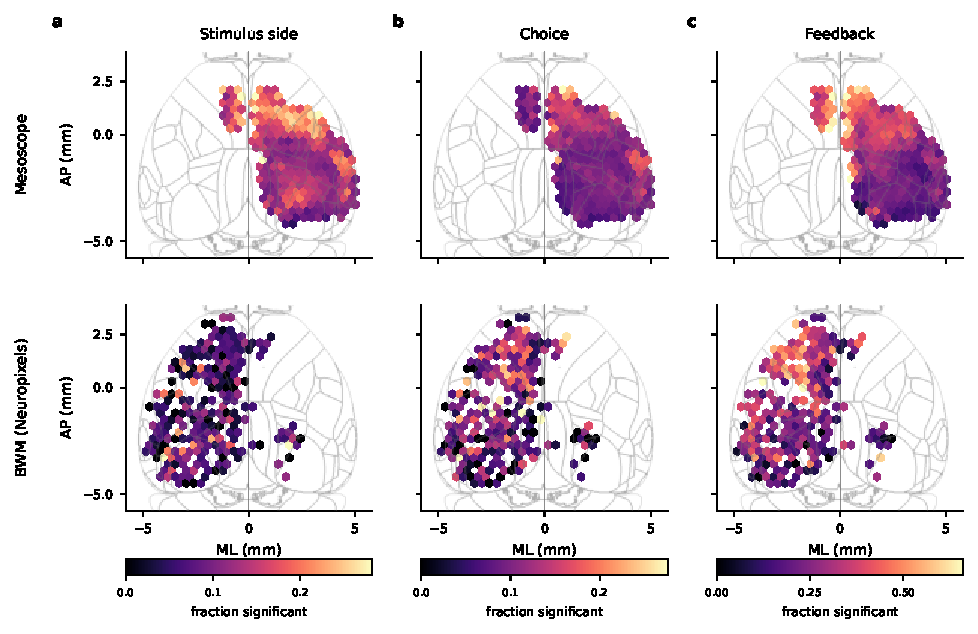
\includegraphics[width=7.00in,height=0.78\textheight,keepaspectratio]{figures/fig3_tuning/dorsal_tuning_unfolded_panels.pdf}
  \caption{Dorsal cortex maps, mesoscope two-photon imaging (top row; deconvolved activity of isocortex neurons, canonical sessions) vs Brain Wide Map Neuropixels recordings (bottom row; good isocortex units, 2023 release). Each neuron is assigned to a hexagonal bin (0.4\,mm vertex to vertex) by its medio-lateral (ML) and antero-posterior (AP) Allen CCF position relative to bregma; both hemispheres shown as recorded. Grey lines: Allen top-view region boundaries. Trials: choice made and reaction time 0.08--2\,s (BWM criteria). Colour scales are shared between the two rows. Single-neuron tuning: the BWM single-cell test (brainwidemap single\_cell\_stats, re-implemented on the GPU and checked against the original), applied identically to both modalities to the mean activity in each window. Mann--Whitney $U$ statistics are computed within condition strata, summed and normalised; the null distribution comes from 3000 permutations of the condition labels within consecutive blocks, and $p$ is the rank of the observed statistic. Mesoscope windows are 0.3\,s long because the frame period is about 0.2\,s. \textbf{a} Fraction of neurons in each bin significantly tuned to stimulus side ($p<0.05$; bins with $\geq$10 neurons pooled across sessions); left vs right stimulus, compared within block $\times$ choice; window $[0, 0.1]$\,s (BWM) or $[0, 0.3]$\,s (mesoscope) relative to stimulus onset. \textbf{b} Same for choice (left vs right turn, within block $\times$ stimulus side); window $[-0.1, 0]$\,s (BWM) or $[-0.3, 0]$\,s (mesoscope) relative to movement onset. \textbf{c} Same for feedback (reward vs error, within block $\times$ stimulus side); window $[0, 0.2]$\,s (BWM) or $[0, 0.3]$\,s (mesoscope) relative to feedback.}
  \label{fig:fig3_tuning}
\end{figure}
